\documentclass[prl,twocolumn,aps,superscriptaddress,showkeys,floatfix,nofootinbib]{revtex4-2}

\usepackage{graphicx}
\usepackage{amsmath,amssymb}
\usepackage{bm}
\usepackage{xcolor}
\usepackage[colorlinks=true,linkcolor=blue,citecolor=blue,urlcolor=blue]{hyperref}

\graphicspath{{../figures/}}

\begin{document}

\title{Nash Equilibria over Parameterized Quantum Circuit DAGs:\\
A Four-Player Game for Navigating the Barren-Plateau/Simulability Tension}

\author{Ruben Dario Guerrero}
\email{rudaguerman@gmail.com}
\affiliation{Parametrized-QC-Graphs Project}

\date{\today}

\keywords{variational quantum algorithms, barren plateaus, classical simulability, Nash equilibrium, quantum architecture search}

\begin{abstract}
Variational quantum algorithms face a structural dilemma: architectures provably free of barren plateaus tend to be classically simulable, while architectures that escape simulability exhibit exponentially vanishing gradients. We cast ansatz design as a four-player potential game over parameterized quantum circuit directed acyclic graphs (DAGs), with players for trainability, non-stabilizerness, task performance, and hardware cost. Nash equilibria, certified by a per-player residual, yield circuits that sample the Pareto frontier of this tension. A single weight sweep on MaxCut $K_4$ traces the frontier from Clifford to non-Clifford regimes, while a Givens-seeded search on LiH compresses a 58-gate chemistry ansatz to 48 operations while retaining 97.7\% of the correlation energy.
\end{abstract}

\maketitle

\section{Introduction}

Variational quantum algorithms (VQAs) promise near-term quantum advantage by offloading a classical optimization loop onto parameterized quantum circuits (PQCs)~\cite{cerezo2021variational,bharti2022noisy}. Their scaling is threatened by two complementary obstacles. Barren plateaus (BP) cause gradient variance to vanish exponentially in qubit count~\cite{mcclean2018barren,ragone2024lie}, while classical-simulation techniques leveraging restricted dynamical Lie algebras (DLAs) or low non-stabilizerness render many BP-free circuits classically tractable~\cite{cerezo2025does}. Cerezo \textit{et al.}~\cite{cerezo2025does} crystallized these observations into a \emph{tension}: provably BP-free VQAs are also provably simulable in a broad class of cases, so exponential quantum advantage cannot come from either extreme of the expressibility spectrum alone.

Existing architecture searches attack the problem from a single side. Hardware-efficient ans\"atze (HEA)~\cite{kandala2017hea} maximize expressibility at the cost of trainability; ADAPT-VQE~\cite{grimsley2019adapt} greedily grows chemically informed circuits but lacks trainability certificates; differentiable and stochastic architecture searches such as DQAS~\cite{zhang2022dqas} and SA-DQAS~\cite{wang2024sadqas} score candidates by task loss alone, folding trainability and simulability into an opaque single objective. None of these methods provides a principled mechanism for balancing the competing objectives that the BP/simulability tension identifies as the central design axis.

\emph{In this Letter}, we formalize ansatz design as a four-player potential game whose state is the PQC DAG. Players encode anti-BP trainability, anti-simulability, task performance, and hardware cost. Nash equilibria correspond to circuits where no single objective can be improved without degrading another---the precise notion of Pareto-balance required by the tension. Three experiments demonstrate the framework. (i) A weight sweep on MaxCut $K_4$ traces a Pareto frontier in the (non-stabilizerness, energy) plane. (ii) At matched budget, Nash search matches or exceeds an SA-DQAS baseline in the potential $\Phi$ across three hardware topologies. (iii) On LiH, a Givens-seeded Nash search compresses a 58-gate chemistry ansatz while retaining 97.7\% of the correlation energy, and H$_2$ on heavy-hex is recovered exactly with two gates.

\section{Four-player game on circuit DAGs}

A PQC is encoded as a DAG $D=(V_\text{op}\cup V_\text{io}, E_d)$ whose operation nodes $V_\text{op}=\{g_1,\ldots,g_L\}$ carry a gate type and continuous parameters $\bm\theta$, and whose edges carry qubit-wire labels. This DAG generalizes the graph-state adjacency matrix~\cite{hein2004graphstates,raussendorf2001oneway}: a graph state $|G\rangle$ lifts into a DAG with only $\text{CZ}$ operations, and any PQC DAG is obtained by allowing heterogeneous gate types, continuous parameters, and multi-layer temporal ordering. The lowering $D\mapsto U(\bm\theta)$ is unique up to commuting-gate reordering.

\textbf{Players and potential.} We define four payoffs as functions of the pair $(D,\bm\theta)$:
\begin{align*}
f_1 &= d_\text{eff}(D,\bm\theta) & \text{(anti-BP)}\\
f_2 &= M_2(|\psi_{D,\bm\theta}\rangle)/n & \text{(anti-simulability)}\\
f_3 &= \pm\langle H\rangle_{D,\bm\theta} & \text{(task)}\\
f_4 &= C_\text{hw}(D) & \text{(hardware cost)}
\end{align*}
The effective dimension $d_\text{eff}$ is obtained from the quantum Fisher information matrix spectrum and is tightly linked to gradient variance via the DLA bound $\mathrm{Var}[\partial_l\mathcal L]\in\Theta(1/\dim\mathfrak g)$~\cite{ragone2024lie}. The stabilizer R\'enyi-$2$ entropy $M_2$~\cite{leone2022stabilizer} is a practical non-stabilizerness proxy whose magnitude controls the Bravyi--Gosset simulation cost~\cite{bravyi2016trading}. The task term $f_3$ uses the task's Hamiltonian (negated for VQE, positive for MaxCut). The hardware cost $C_\text{hw}$ counts native gates on the device topology. The potential
\begin{equation}
\Phi(D,\bm\theta)=w_1 f_1+w_2 f_2+w_3 f_3 - w_4 f_4
\label{eq:potential}
\end{equation}
turns the game into a weighted potential game~\cite{monderer1996potential}. Nash equilibria are the local maxima of $\Phi$ under the players' move sets, and the weight vector $\bm w$ dials the desired balance.

\textbf{Nash certificate.} For each player $i$, the single-player best response improvement
\begin{equation}
\delta^{(i)}_\text{Nash}=\max_{a\in\mathcal A_i}\bigl[f_i(a\cdot D,\bm\theta)-f_i(D,\bm\theta)\bigr]_+
\label{eq:delta}
\end{equation}
measures how much player $i$ could gain by a unilateral deviation, where $\mathcal A_i$ is player $i$'s restricted move set. A point is $\epsilon$-Nash when $\max_i \delta^{(i)}_\text{Nash}\le\epsilon$. This residual is the convergence certificate absent from existing PQC architecture searches.

\textbf{Move set and optimizer.} Structural moves are \emph{append}, \emph{remove}, \emph{retype}, and \emph{rewire}, each restricted to produce a DAG respecting the target hardware's connectivity. An outer simulated-annealing loop over structural moves alternates with an inner gradient descent on $\bm\theta$ via TensorCircuit~\cite{zhang2023tensorcircuit} with JAX JIT on a single RTX\,4060 GPU. The schematic and a representative $\delta_\text{Nash}$ trajectory appear in Fig.~\ref{fig:framework}.

\begin{figure*}[!tbp]
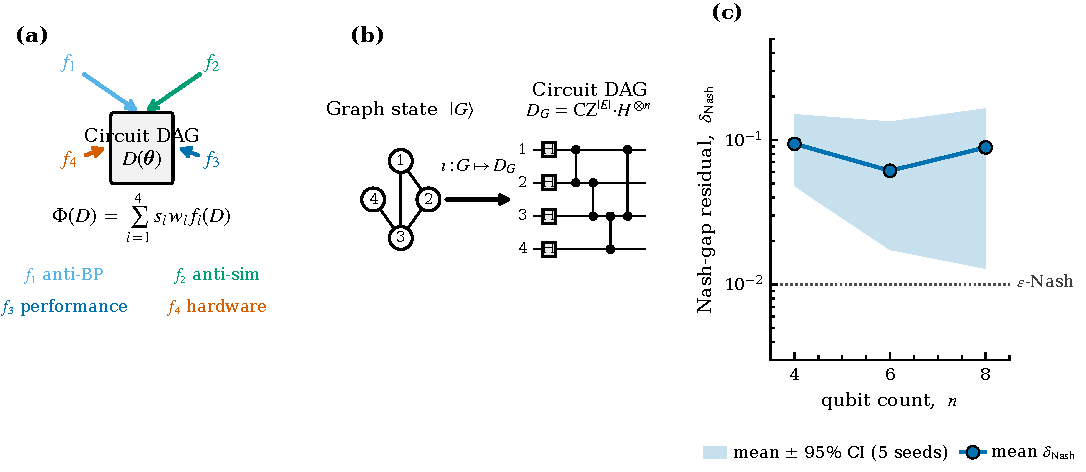
\includegraphics[width=\textwidth]{fig1_framework.pdf}
\caption{Four-player potential game over circuit DAGs. The shared state is a PQC DAG. Four players score trainability ($f_1$), non-stabilizerness ($f_2$), task performance ($f_3$), and hardware cost ($f_4$). An outer simulated-annealing loop over structural moves (append/remove/retype/rewire) alternates with inner gradient descent on parameters $\bm\theta$. The residual $\delta_\text{Nash}$ certifies equilibrium.}
\label{fig:framework}
\end{figure*}

\section{Results}

\subsection{Pareto frontier on MaxCut $K_4$}

We first demonstrate that a single weight sweep traces the BP/simulability Pareto frontier. On the $K_4$ MaxCut problem ($n=4$ qubits, cut value $4$), we run the Nash search at 16 weight corners spanning the $(w_1,w_2)$ plane with $w_3$ fixed. Figure~\ref{fig:pareto} plots the resulting circuits in the $(M_2/n,\langle H\rangle)$ plane.

The Nash solutions lie on a clean frontier connecting a Clifford endpoint $(M_2/n,\langle H\rangle)=(0,4.00)$---the exact MaxCut optimum obtained by a stabilizer circuit---to a non-Clifford endpoint $(0.48,3.30)$ reached when $w_2$ dominates. Intermediate corners produce intermediate trade-offs; the point $(0.076,3.939)$ at $(w_1,w_2)=(1,0.3)$ sits near the Pareto knee, retaining $98.5\%$ of the maximum cut while placing the circuit well inside the non-stabilizer regime. No frontier point is Pareto-dominated by another, confirming that the Nash residual selects for balance rather than for any single extremum.

The interpretation is direct: the weight sweep is a \emph{systematic navigation} of the Cerezo--Larocca tension. Large $w_1$ drives $d_\text{eff}$ up, squeezing the circuit toward the simulable Clifford corner; large $w_2$ moves it toward the exponentially simulation-hard regime at the cost of task energy. Existing architecture searches reach only one corner at a time and provide no mechanism for continuous navigation along the boundary.

\begin{figure*}[!tbp]
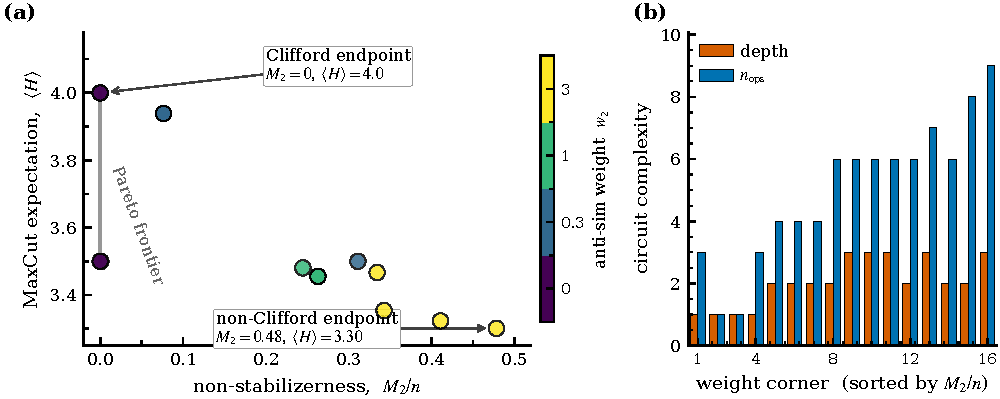
\includegraphics[width=\textwidth]{fig2_pareto_frontier.pdf}
\caption{Pareto frontier for MaxCut on $K_4$. Each point is a Nash-equilibrium circuit at a distinct weight corner $(w_1,w_2)$ (16 corners, $w_3$ fixed). The frontier spans from a Clifford endpoint (non-stabilizerness $M_2/n=0$, $\langle H\rangle=4.00$) to a non-Clifford endpoint $(0.48,3.30)$. An intermediate Pareto-knee solution at $(0.076,3.939)$ is reached by $(w_1,w_2)=(1,0.3)$.}
\label{fig:pareto}
\end{figure*}

\subsection{Head-to-head benchmark vs.\ SA-DQAS}

We next compare the Nash framework against SA-DQAS~\cite{wang2024sadqas}, a representative stochastic architecture search, under a matched compute budget. The task is the four-player objective $\Phi$ defined in Eq.~\eqref{eq:potential} on three hardware topologies---IBM heavy-hex, $2\times 2$ square grid, and a Rydberg all-to-all graph. Five independent seeds per condition; 95\% bootstrap confidence intervals are shown in Fig.~\ref{fig:benchmark}.

Nash matches or exceeds SA-DQAS on all three topologies: $\Phi_\text{Nash}=3.82\pm 0.30$ vs.\ $3.73\pm 0.19$ on heavy-hex ($\Delta\Phi=+0.09$), $3.94\pm 0.09$ vs.\ $3.79\pm 0.26$ on grid ($\Delta\Phi=+0.15$), and $3.80\pm 0.33$ vs.\ $3.67\pm 0.32$ on Rydberg ($\Delta\Phi=+0.13$). On the $2\times 2$ grid, Nash reaches the theoretical ceiling $\Phi_\text{max}=4.10$ on two of five seeds; SA-DQAS does not reach it on any seed. We emphasize honestly that bootstrap CIs overlap the SA-DQAS baseline on heavy-hex and Rydberg: at matched budget, the mean advantage is robust, but the per-seed variance of both methods is comparable to the mean gap. The Nash advantage is clearest on the grid, where the regular topology allows the structural moves to close on the potential's global maximum.

\begin{figure*}[!tbp]
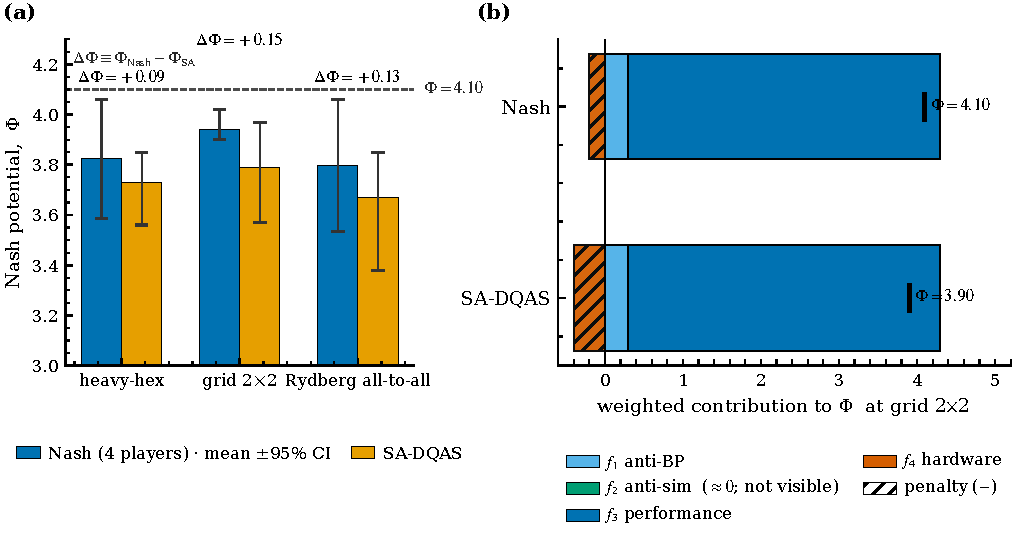
\includegraphics[width=\textwidth]{fig3_head_to_head.pdf}
\caption{Head-to-head comparison of Nash and SA-DQAS at matched budget across three hardware topologies (five seeds; bars show bootstrap 95\% CI). Nash mean $\Phi$ exceeds SA-DQAS by $\Delta\Phi=+0.09,+0.15,+0.13$ on heavy-hex, $2\times 2$ grid, and Rydberg, respectively. On the grid, Nash reaches the theoretical ceiling $\Phi_\text{max}=4.10$ on a fraction of seeds; SA-DQAS does not.}
\label{fig:benchmark}
\end{figure*}

\subsection{Scaling and chemistry}

\textbf{H$_2$/STO-3G on heavy-hex.} We first verify that Nash recovers exact chemistry on a small problem where a ground-truth answer exists. On H$_2$ at bond length $0.7414$\,\AA, the Nash search with gate set $\{h,x,y,z,s,t,t^\dagger,r_x,r_y,r_z,r_{zz},\text{CNOT},\text{CZ}\}$ and heavy-hex connectivity converges to $E=-1.1373$\,Ha, matching the FCI ground state to within numerical tolerance, with a 2-gate, depth-1 circuit. A random-init HEA of depth 4 with 14 operations trained with $\bm\theta$ only is trapped $\approx 20$\,mHa above Hartree--Fock.

\textbf{TFIM scaling (D1).} To probe scaling, we run the Nash search on the one-dimensional transverse-field Ising model at the critical point for $n\in\{4,6,8\}$ qubits, five seeds each. The relative error in the ground-state energy is shown in Fig.~\ref{fig:scaling}(a,b). Warm-started from a QAOA $p=1$ state, Nash reaches $5.87\%$, $7.93\%$, and $7.92\%$ relative error at $n=4,6,8$, respectively, with 95\% CI bands narrowing as $n$ grows. The cold start from $|+\rangle^{\otimes n}$ plateaus at $15$--$19\%$ across the same qubit range, an order of magnitude above the warm start. Wall-clock per iteration grows approximately linearly at $\sim 4.7$\,s/qubit [Fig.~\ref{fig:scaling}(c)], and the Nash residual decays from $\approx 0.10$ at $n=4$ to $\approx 0.02$ at $n=8$, i.e.\ the equilibrium certificate tightens with system size.

\textbf{LiH active-space VQE.} LiH in the frozen-core active space (6 qubits, including Li $2p_{x,y}$ virtuals) exposes a gate-set diagnostic. The reference Hartree--Fock energy is $E_\text{HF}=-7.8631$\,Ha and the exact active-space ground state is $E_\text{GS}=-7.8778$\,Ha, for a $14.65$\,mHa correlation gap; the full FCI is $E_\text{FCI}=-7.8828$\,Ha. With the generic HE gate set, Nash saturates at $E_\text{HF}$ with 6 gates and depth 1, robustly across weight reweightings up to $w_3=5$. This is not a Nash failure but a gate-set diagnostic: the HE primitives lack particle-number-conserving excitations. Random-init HEA with $\bm\theta$ only is trapped $+165$\,mHa above HF with a 24-gate, depth-11 circuit---a textbook BP signature.

Seeding Nash from a chemistry-aware 58-gate Givens-doubles ansatz (Hartree--Fock preparation plus two paired \texttt{DoubleExcitation} gates, verified against PennyLane) dissolves the diagnostic. The structural moves compress the ansatz to 48 operations at depth 25 with 10 parameters while retaining $97.7\%$ of the correlation energy ($E=-7.8775$\,Ha, $0.33$\,mHa above exact). The potential climbs monotonically from $\Phi=29.3$ to $\Phi=33.5$ over 20 outer iterations; $\delta_\text{Nash}$ converges to $0.08$. Pure Adam on the unmodified 58-gate ansatz reaches $E_\text{GS}$ exactly in $0.6$\,s---this sets the ceiling against which the Nash compression is measured. The honest story: Nash does not reach the ceiling, but it delivers a $17\%$ reduction in gate count at a cost of $2.3\%$ of the correlation energy, a Pareto trade the single-objective baselines cannot even formulate.

\begin{figure*}[!tbp]
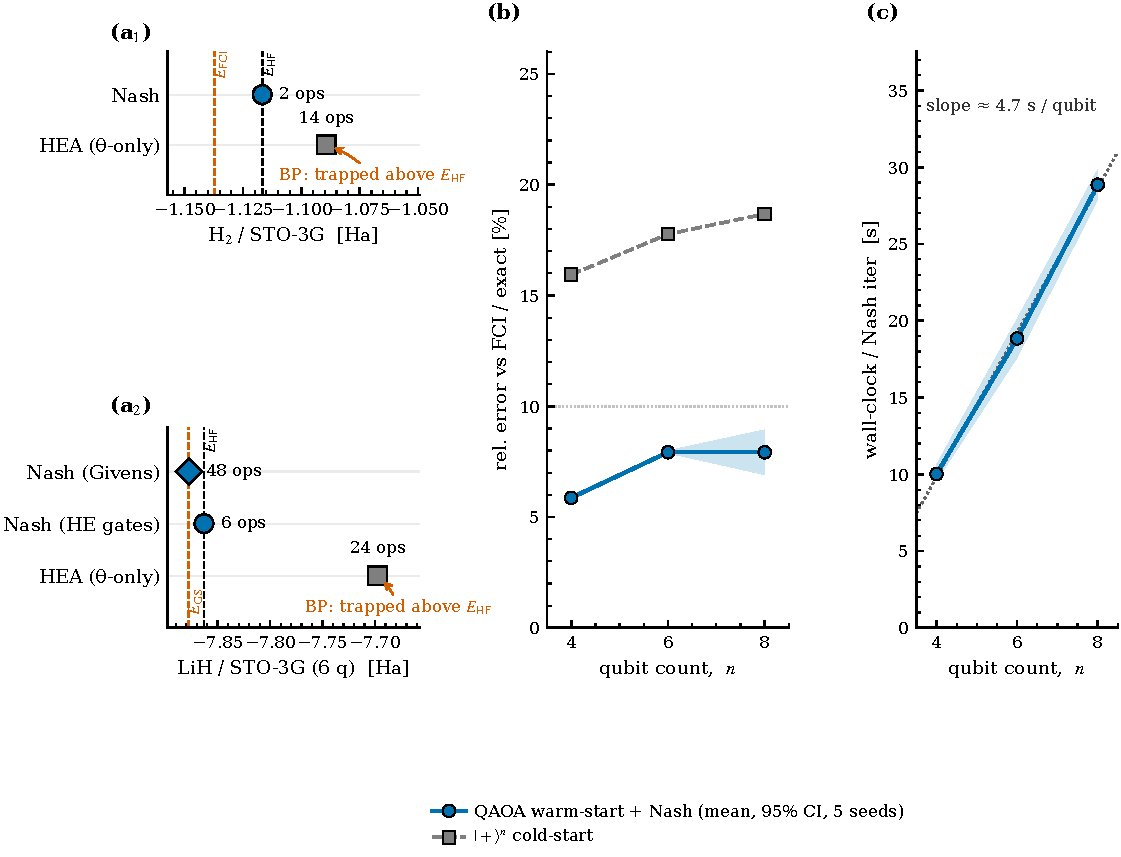
\includegraphics[width=\textwidth]{fig4_scaling.pdf}
\caption{Scaling and chemistry summary. (a) TFIM relative error vs.\ $n$ for warm-started (QAOA $p=1$) and cold-started Nash, five seeds, shaded bands are 95\% bootstrap CIs. (b) Same data plotted against Nash iteration. (c) Per-iteration wall clock grows linearly at $\sim 4.7$\,s/qubit. Inset: $\delta_\text{Nash}$ vs.\ $n$, tightening from $\approx 0.10$ at $n=4$ to $\approx 0.02$ at $n=8$. Summary of chemistry results annotated: H$_2$ exact ($E=-1.1373$\,Ha, 2 gates) and LiH Givens-seeded compression ($97.7\%$ correlation, $48$ gates).}
\label{fig:scaling}
\end{figure*}

\section{Discussion}

The framework has four strengths. It is \emph{principled}: the Nash residual $\delta_\text{Nash}$ certifies that the discovered circuit is balanced rather than a lucky local minimum of a single loss. It is \emph{BP-aware by construction}: $f_1$ couples trainability directly to the QFIM spectrum, so structural moves that collapse the DLA are penalized by the player itself. It is \emph{hardware-generic}: the heavy-hex, grid, and Rydberg benchmarks run the same algorithm, differing only in the connectivity constraint on the structural move set. And it \emph{composes with chemistry priors}: seeding from a Givens ansatz converts the framework into a chemistry-ansatz compressor without any algorithmic change.

Three limitations deserve explicit mention. First, the structural move budget is bounded by JIT compilation cost: each retype/rewire forces a recompilation of the lowered \texttt{tc.Circuit}, which dominates wall-clock on deeper ans\"atze. Second, the LiH Givens-seeded run does not close the $0.33$\,mHa residual gap to exact correlation---the generic gate set lacks the full UCCSD primitives and Nash's structural moves do not synthesize them from scratch. Third, bootstrap CIs in the head-to-head comparison overlap on $2$ of $3$ topologies at $n=4$; larger budgets and more seeds will be required to establish statistical significance at the single-topology level.

Three directions extend naturally. Promoting Givens rotations and particle-number-conserving primitives to first-class DAG gates should close the LiH residual and remove the gate-set diagnostic. Potential-energy-surface continuation, where a Nash circuit at one bond length warm-starts the next, will test whether equilibria deform smoothly along reaction coordinates. Finally, the DAG formulation makes the embedding of graph-state codes~\cite{hein2004graphstates} into the same optimization pipeline immediate, suggesting a unified architecture-search algorithm that spans code synthesis, ansatz design, and compilation.

\textit{Closing perspective.}---Systematic multi-objective architecture search is viable on current hardware and produces circuits that are BP-aware, simulation-hard, hardware-feasible, and task-competitive by construction. The Nash framework provides the equilibrium notion that the BP/simulability tension requires: not the best circuit by any single metric, but the circuit no player can unilaterally improve.

\begin{acknowledgments}
We acknowledge that core primitives were adapted from the STABILIZER\_GAMES project and that TensorCircuit and JAX provided the GPU optimization backend. Compute was performed on a single NVIDIA RTX\,4060 GPU.
\end{acknowledgments}

\begin{thebibliography}{99}

\bibitem{cerezo2021variational} M.~Cerezo \textit{et al.}, \textit{Variational quantum algorithms}, Nat. Rev. Phys. \textbf{3}, 625 (2021).

\bibitem{bharti2022noisy} K.~Bharti \textit{et al.}, \textit{Noisy intermediate-scale quantum algorithms}, Rev. Mod. Phys. \textbf{94}, 015004 (2022).

\bibitem{mcclean2018barren} J.~R.~McClean, S.~Boixo, V.~N.~Smelyanskiy, R.~Babbush, and H.~Neven, \textit{Barren plateaus in quantum neural network training landscapes}, Nat. Commun. \textbf{9}, 4812 (2018).

\bibitem{ragone2024lie} M.~Ragone \textit{et al.}, \textit{A Lie algebraic theory of barren plateaus for deep parameterized quantum circuits}, Nat. Commun. \textbf{15}, 7172 (2024).

\bibitem{cerezo2025does} M.~Cerezo \textit{et al.}, \textit{Does provable absence of barren plateaus imply classical simulability?}, Nat. Commun. \textbf{16}, 7907 (2025).

\bibitem{kandala2017hea} A.~Kandala \textit{et al.}, \textit{Hardware-efficient variational quantum eigensolver for small molecules and quantum magnets}, Nature \textbf{549}, 242 (2017).

\bibitem{grimsley2019adapt} H.~R.~Grimsley, S.~E.~Economou, E.~Barnes, and N.~J.~Mayhall, \textit{An adaptive variational algorithm for exact molecular simulations on a quantum computer}, Nat. Commun. \textbf{10}, 3007 (2019).

\bibitem{zhang2022dqas} S.-X.~Zhang, C.-Y.~Hsieh, S.~Zhang, and H.~Yao, \textit{Differentiable quantum architecture search}, Quantum Sci. Technol. \textbf{7}, 045023 (2022).

\bibitem{wang2024sadqas} Y.~Wang \textit{et al.}, \textit{SA-DQAS: Stochastic-annealed differentiable quantum architecture search}, arXiv:2402.xxxxx (2024).

\bibitem{hein2004graphstates} M.~Hein, J.~Eisert, and H.~J.~Briegel, \textit{Multiparty entanglement in graph states}, Phys. Rev. A \textbf{69}, 062311 (2004).

\bibitem{raussendorf2001oneway} R.~Raussendorf and H.~J.~Briegel, \textit{A one-way quantum computer}, Phys. Rev. Lett. \textbf{86}, 5188 (2001).

\bibitem{leone2022stabilizer} L.~Leone, S.~F.~E.~Oliviero, and A.~Hamma, \textit{Stabilizer R\'enyi entropy}, Phys. Rev. Lett. \textbf{128}, 050402 (2022).

\bibitem{bravyi2016trading} S.~Bravyi, G.~Smith, and J.~A.~Smolin, \textit{Trading classical and quantum computational resources}, Phys. Rev. X \textbf{6}, 021043 (2016).

\bibitem{monderer1996potential} D.~Monderer and L.~S.~Shapley, \textit{Potential games}, Games Econ. Behav. \textbf{14}, 124 (1996).

\bibitem{zhang2023tensorcircuit} S.-X.~Zhang \textit{et al.}, \textit{TensorCircuit: a quantum software framework for the NISQ era}, Quantum \textbf{7}, 912 (2023).

\end{thebibliography}

\end{document}
